% Construction : courbe en cloche centrée en μ, d'écart type σ.
%   Échantillonnée sur -3.4σ..3.4σ par y = 2.2 exp(-t²/2), t en écarts types.
%   Repères à μ et μ ± σ ; la flèche mesure σ, l'écart entre le centre et le
%   point d'inflexion. Les intervalles à 68 %, 95 % et 99,7 % ne sont pas
%   figurés : ce chapitre les admet, et une figure ne comblerait pas ce manque.
% SVG : x = 150 + 40t, y = 120 - 90 exp(-t²/2).
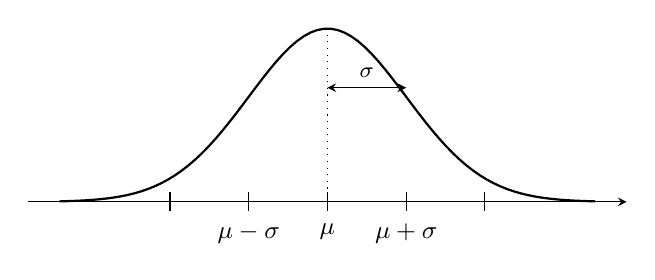
\begin{tikzpicture}[scale=1, >=stealth, every node/.style={font=\small}]
  \draw[->] (-3.8, 0) -- (3.8, 0);
  \draw[domain=-3.4:3.4, samples=80, thick] plot (\x, {2.2*exp(-\x*\x/2)});
  \foreach \t in {-2,-1,0,1,2} \draw (\t, 0.12) -- (\t, -0.12);
  \draw[dotted] (0, 0) -- (0, 2.2);
  \draw[<->] (0, 1.45) -- (1, 1.45) node[midway, above, font=\footnotesize] {$\sigma$};
  \node[below] at (0, -0.15) {$\mu$};
  \node[below] at (1, -0.15) {$\mu + \sigma$};
  \node[below] at (-1, -0.15) {$\mu - \sigma$};
\end{tikzpicture}
